\item{Area Scanning}
\begin{itemize}
\item{Description of mission}
The course will be divided into 10x10 square sections, each with a width of about 31 m. The sections will be indexed as (i, j), where i goes from 0 to 9 starting at south and going north, and j goes from 0 to 9 starting at west and going east. From the time the boat enters the first section and within a time of 90 minutes, the boat shall pass through as many square sections as possible. The score for the area scanning contest will be calculated as:
P = Npassed/10
where Npassed is the number of entered sections.
The score will be multiplied with a factor determined from oceanographic measurements provided for each visited section. Depth (m), water temperature (\textcelsius), air temperature (\textcelsius), water salinity (\%), conductivity (S/cm), chlorophyll (ug/l), ammonium (mg/l), nitrate (mg/l), chloride (mg/l) and total dissolved solids (mg/l) can be provided. Inclusion of depth data will add 0.2 to the multiplication factor, the other measurements each add 0.1. The multiplication factor is 1.0 initially, and the maximum that can be achieved is 1.5. Each team shall provide data on the team’s performance to the Race Committee within 5 hours after the start of their slot time. The data shall be in XML, specified by the schema below. The data will contain the team name. For each entered square section the section’s indices are required along with a UTC timestamp and corresponding coordinates using <gml:pos> property in WGS-84 (EPSG:4326). Optionally the oceanographic data can be added. Each entered section shall be added only once to the XML data.
\item{algorithm for Area Scanning}
Actually, for the contest area scanning, the Race Committee decided to do the scoring by themselves, but they ask us to verify the GPS data submitted by the teams with XML format with data gathered by our trackers. Fortunately, Åland University of Applied Sciences(ÅUAS) had a python program which can analyse the submitted XML file and then generate a JSON file(which contains all the useful data and this file is easy to be handled by ruby on rails). And then I based on this JSON file, compare the data with the correspondent tracker's data to check if the gaps of positions were under the tolerance. In order to accomplish this task, several steps were adopted:
\begin{enumerate}
\item The participated team should uploading their XML file to their robot's page

(robot\#IdOfTheirRobot). And also I added a time stamp to record the time when the team submitted their XML file because the team should upload their XML file in 5 hours since they had finished their attempts.
\item With python program(provided by Conny Ljunggren, ÅUAS), I need to generate a JSON file manually. Also I had looked into the python program, in fact the python program used a module called "xml.etree.ElementTree", the key point of this program is using this module to analyse XML file. Unfortunately, I did not find any similar module in Ruby to analyse the XML file, but it was also feasible in ruby. It was just like a compilation project, the code source is XML file, and then the target file is JSON file, so then if we define the grammar of XML, define the lexer and Backus Normal Form(BNF), from the Backus Normal Form(BNF), create the parser to analyse the code source, and store all the separate data in the node of Abstract Syntax Tree(AST), then either by using the visitor pattern, or mix erb with visitor pattern, we can generate the target code finally. Since we did not have so much more time, I did not realize this function.
\item Based on the JSON file, ruby could import the JSON file directly, then I can compare the GPS data to the data in our web site and calculate the difference between the two sets of data. Because all the unities of GPS data are in degree, which are incomprehensible for humans, then I transfer the unity in degree to the unity in meter by using the algorithm proposed by this site: 
http://www.movable-type.co.uk/scripts/latlong.html

\begin{figure}[h!]
    \centering
    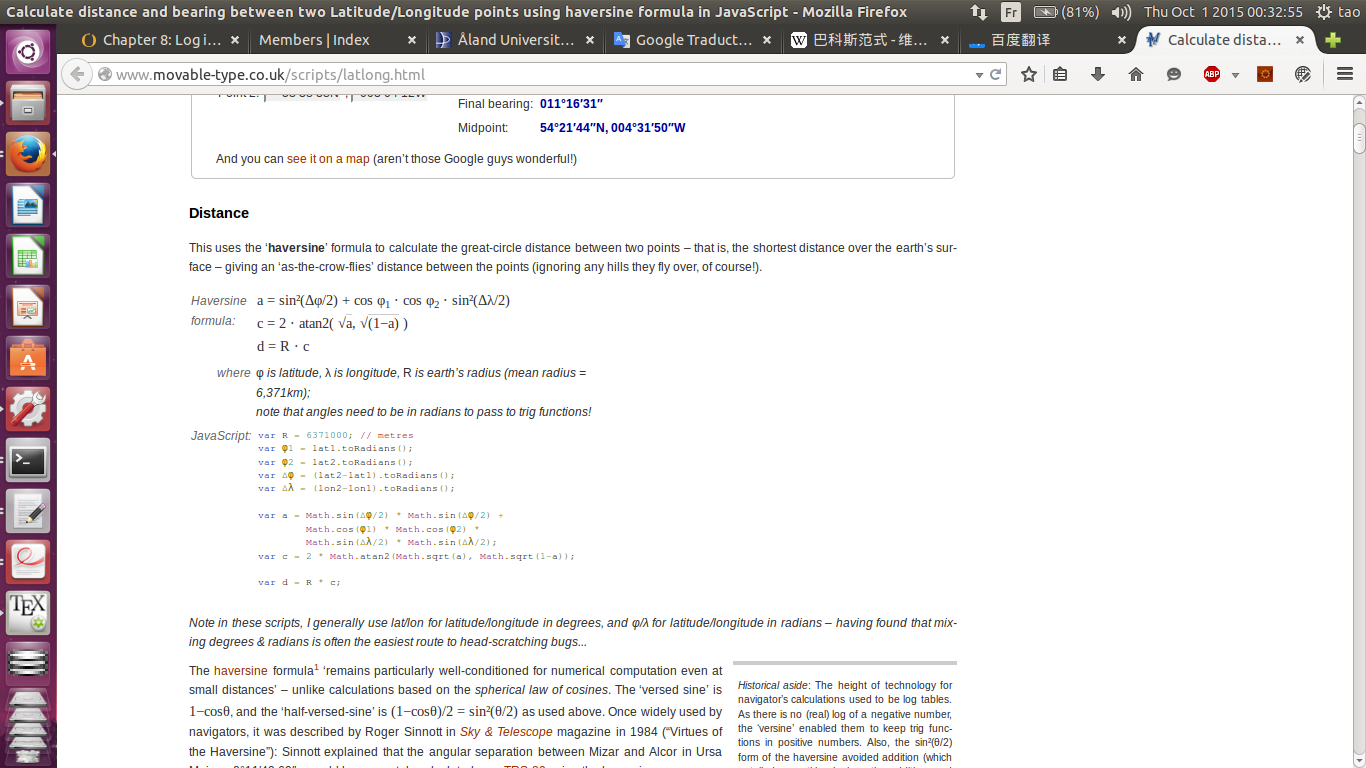
\includegraphics[width=12cm]{distanceformula.png}
    \caption{latitude longitude to meter formula from Internet}
    \label{fig-sample}
\end{figure}
And also I had tried the official contest's buoys positions. In fact, the Race Committee declared officially the distance between two buoys is about 31m [(60.1050,19.9500);(60.1080,19.9500)], and from the formula, I obtain the distance is a little more than 30m, so the gap is less than 1m which is acceptable by the GPS precision.
\item After the comparison, in ruby there are three possibilities(JSON/YAML/XML) to display the result, finally I choose XML not only to keep coherent with what they submitted, but also easy to read for users. As a matter of fact, files are also like any other resource in the web site(like views), according to the path in the rails application, we can visit the file by typing the url Rails.root/FilePath.
\end{enumerate}
 
\end{itemize}